\newpage


\section{Results}
\label{fbg_results}

\begin{figure}[!h]
\centering
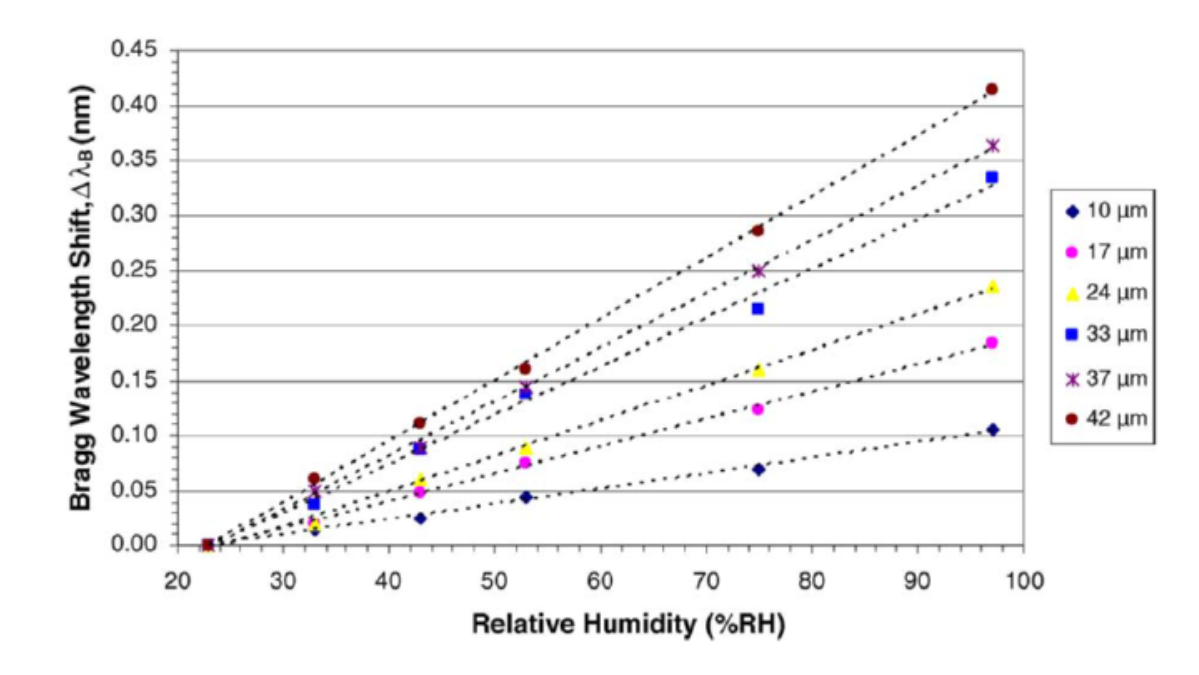
\includegraphics[width=0.85\columnwidth]{Chapter5/images/yeo_coating.png}
\caption{Controls architecture for the temperature and humidity sensor measurement}
\label{fig:fos_coating0}
\end{figure}

\begin{figure}[!h]
\centering
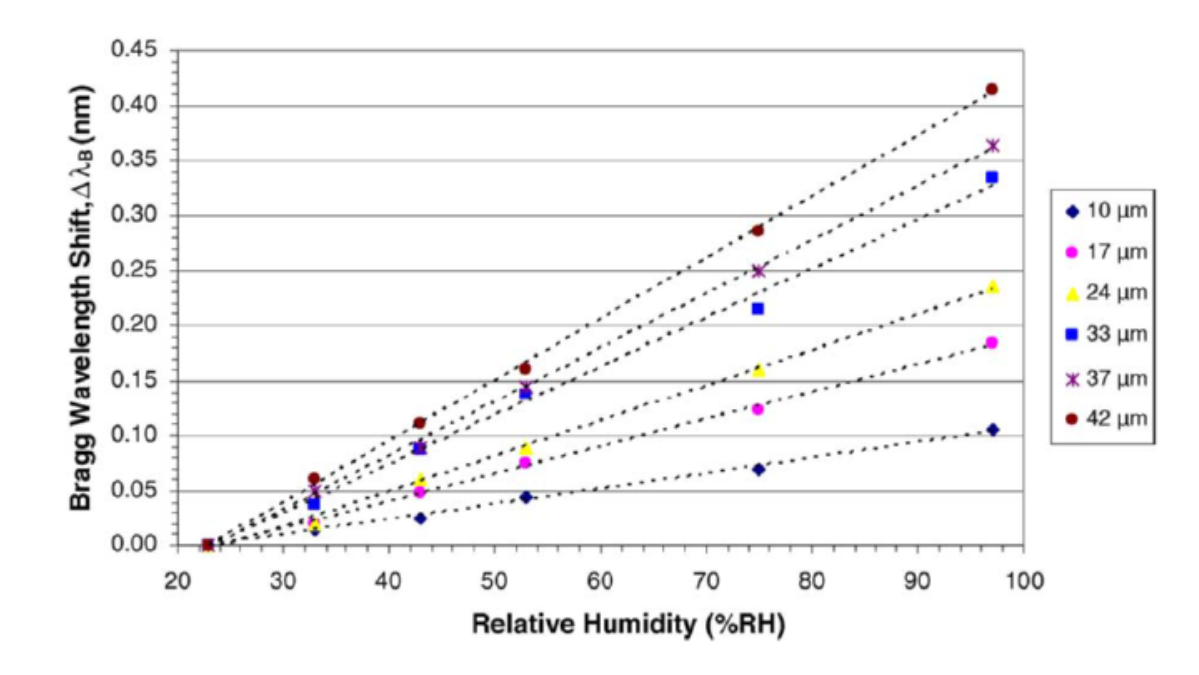
\includegraphics[width=0.85\columnwidth]{Chapter5/images/yeo_coating.png}
\caption{Controls architecture for the temperature and humidity sensor measurement}
\label{fig:fos_coating}
\end{figure}


\begin{figure}[!h]
\centering
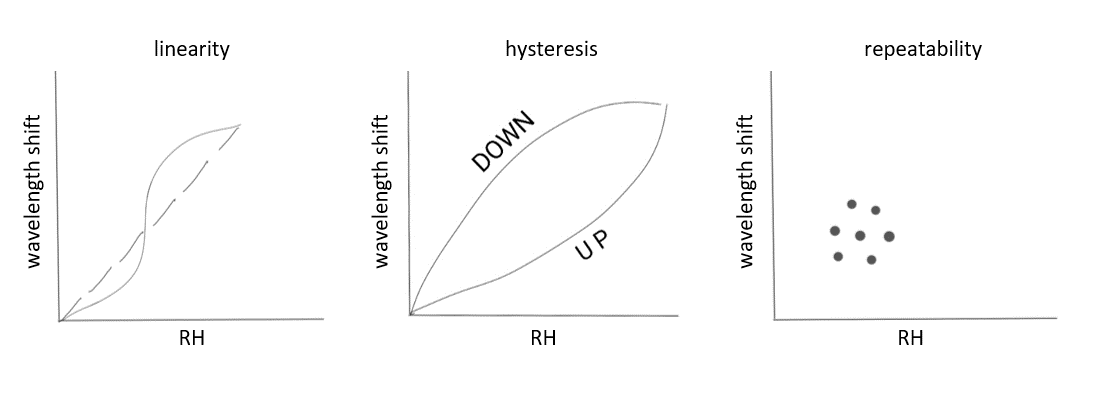
\includegraphics[width=0.85\columnwidth]{Chapter5/images/uncerainty.png}
\caption{Different contributions to the sensor's accuracy}
\label{fig:accuracy}
\end{figure}
\subsection{Characterization of RH FOS}

\begin{figure}[!h]
\centering
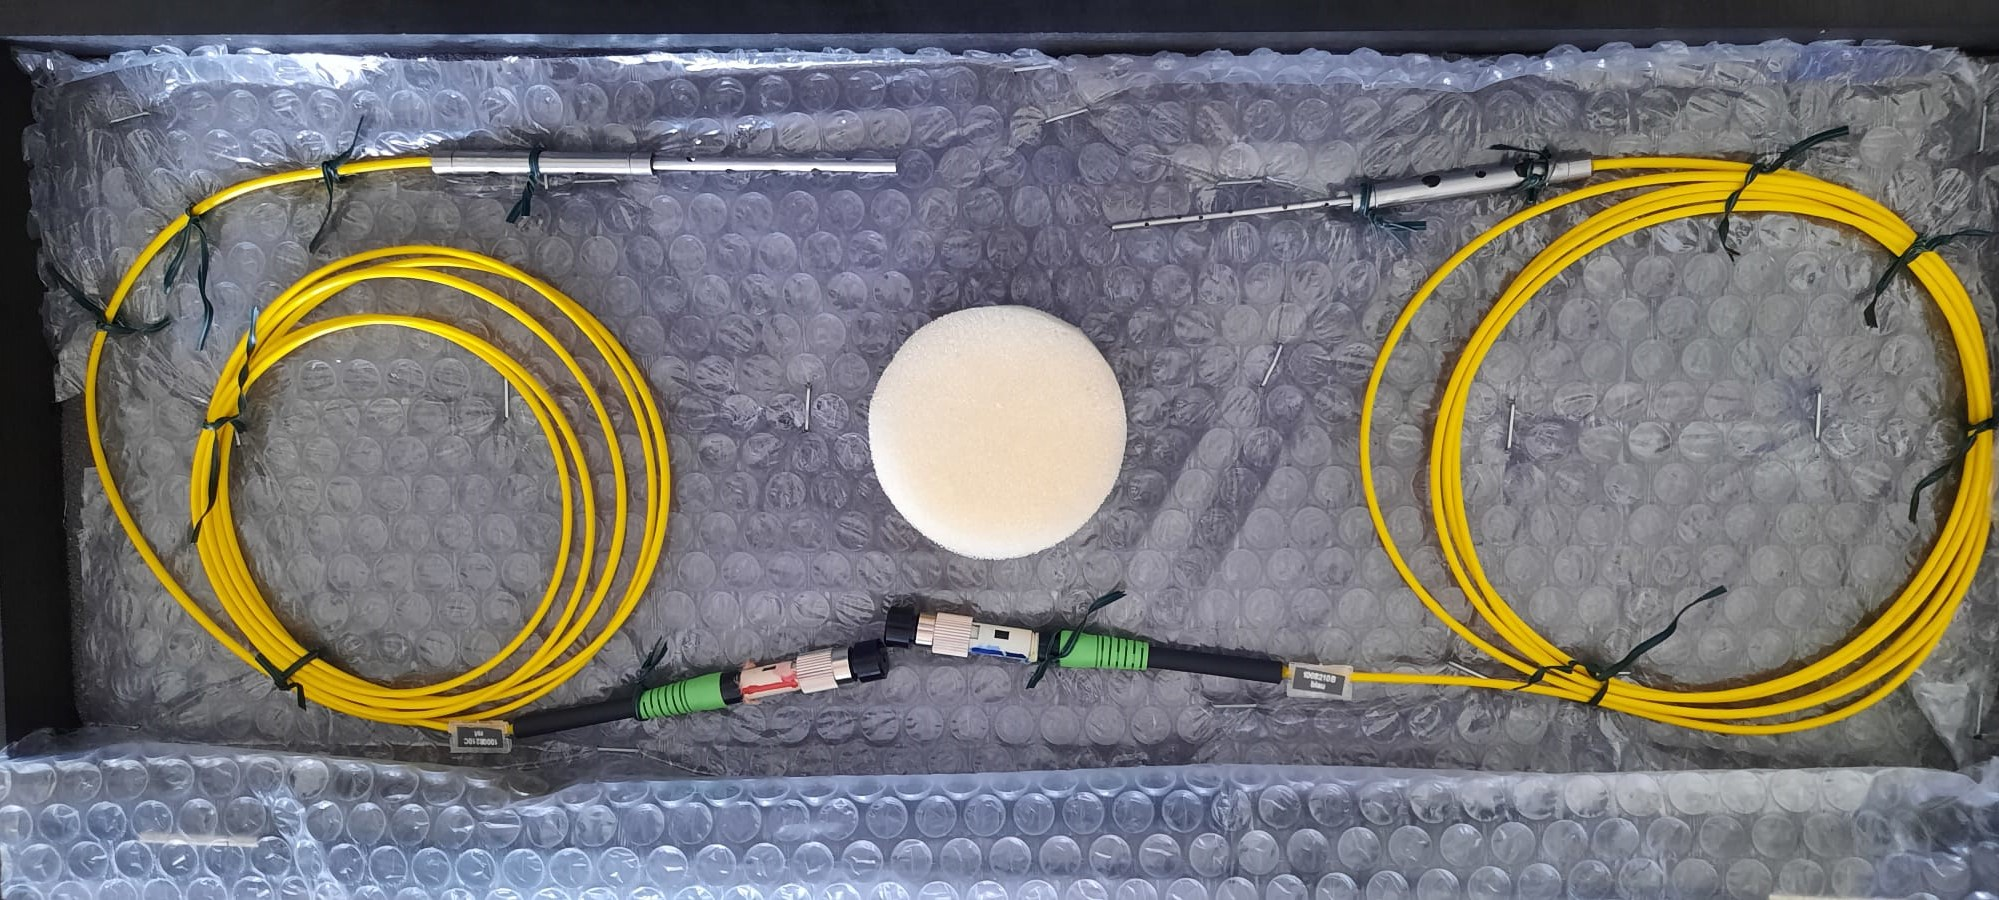
\includegraphics[width=0.65\columnwidth]{Chapter5/images/single1.jpeg}
\caption{Hygrometer (temperature and humidity sensitive FBG inscribed into the same fiber)}
\label{fig_single_photo}
\end{figure}

\begin{figure}[!h]
\centering
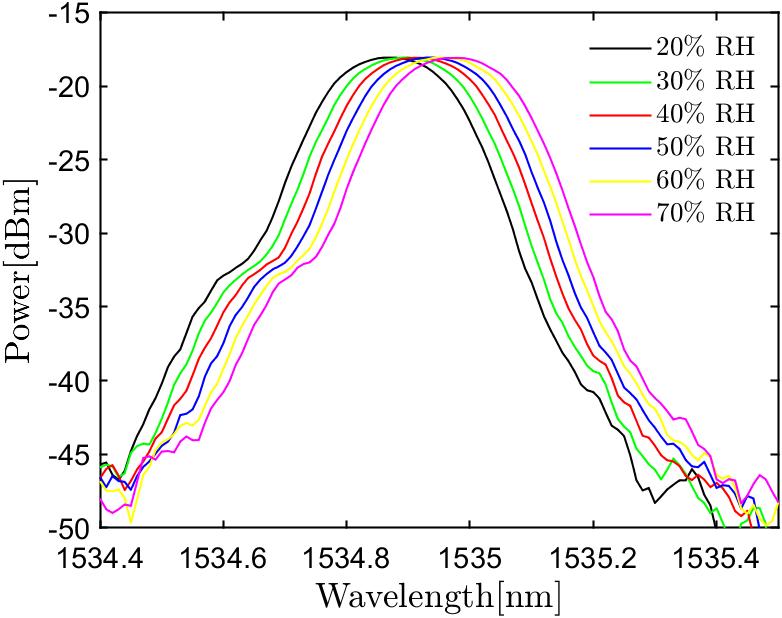
\includegraphics[width=0.6\columnwidth]{Chapter5/images/rh.png}
\caption{Humidity induced Bragg wavelength shift for the single RH+T sensor}
\label{fig_single_wavelength}
\end{figure}


\begin{figure}[!h]
\centering
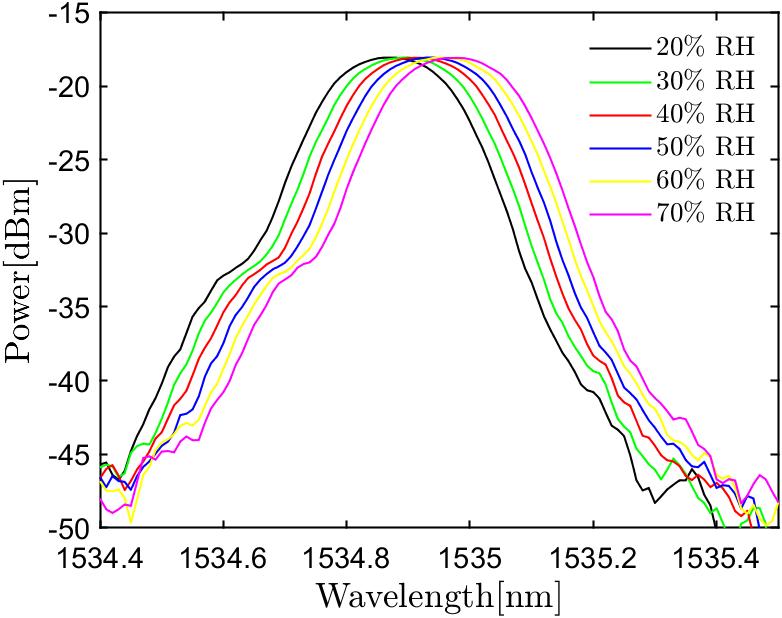
\includegraphics[width=0.6\columnwidth]{Chapter5/images/rh.png}
\caption{Humidity induced Bragg wavelength shift for the hygrometer}
\label{fig_single_wavelength}
\end{figure}


\begin{figure}[!h]
\centering
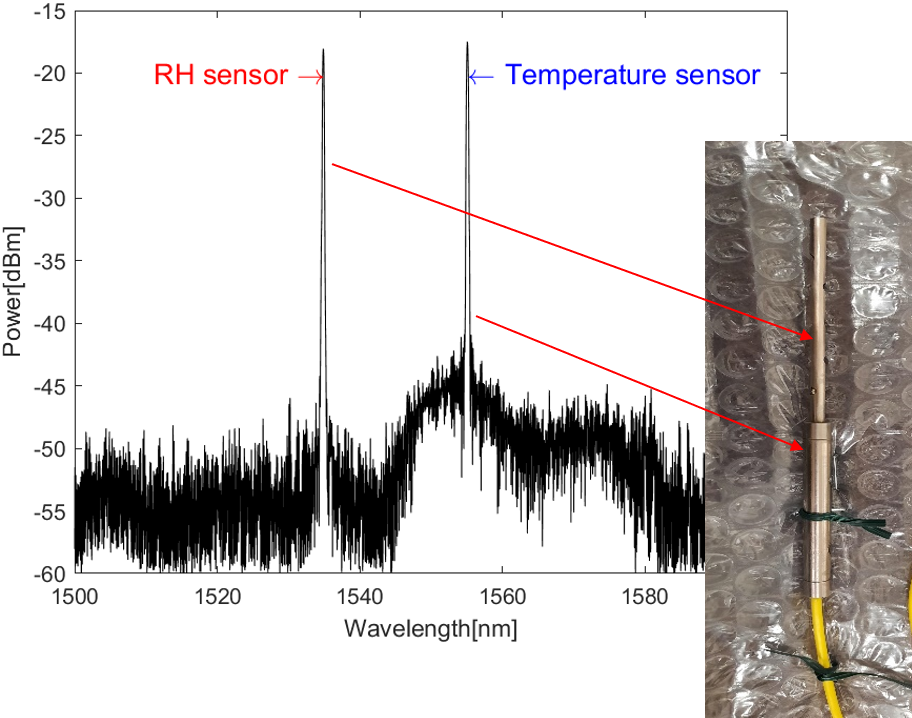
\includegraphics[width=0.6\columnwidth]{Chapter5/images/hygr.png}
\caption{Hysteresis}
\label{fig_hygrometer1}
\end{figure}


\begin{figure}[!h]
\centering
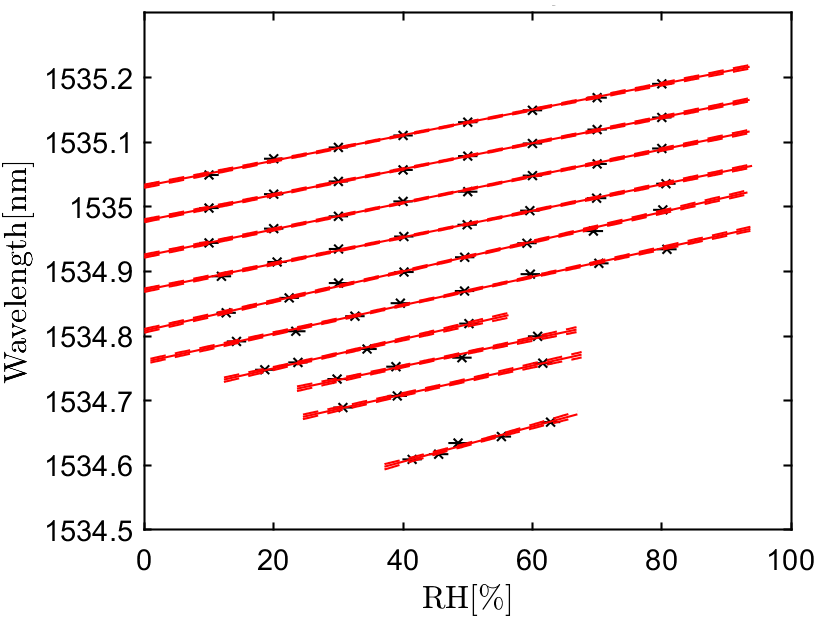
\includegraphics[width=0.6\columnwidth]{Chapter5/images/RHS.png}
\caption{Calibration curves for the hygrometer}
\label{fig_single_calibration}
\end{figure}


\begin{figure}[!h]
\centering
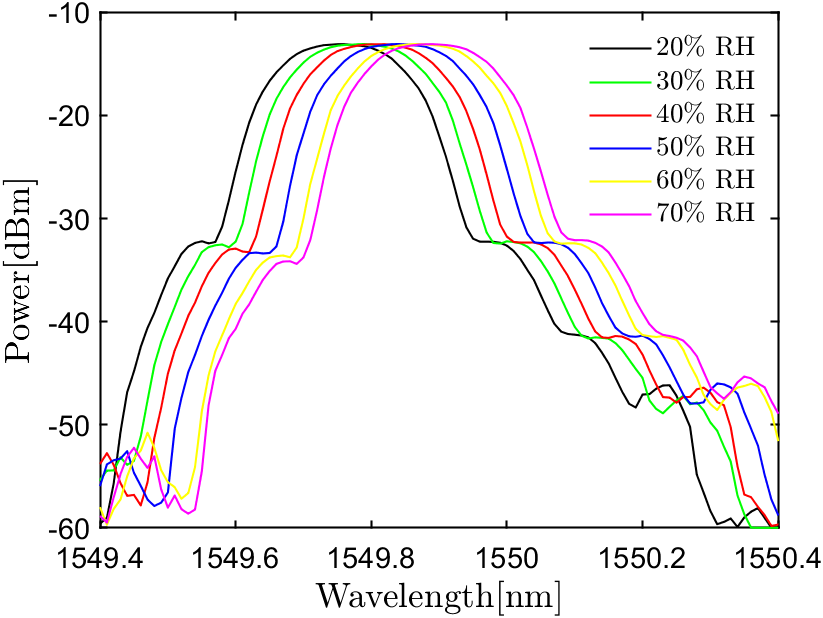
\includegraphics[width=0.6\columnwidth]{Chapter5/images/rh_array2.png}
\caption{Humidity induced Bragg wavelength shift for the sensors array}
\label{fig_single_calibration}
\end{figure}

\subsection{Calibration}

\begin{figure}[!h]
\centering
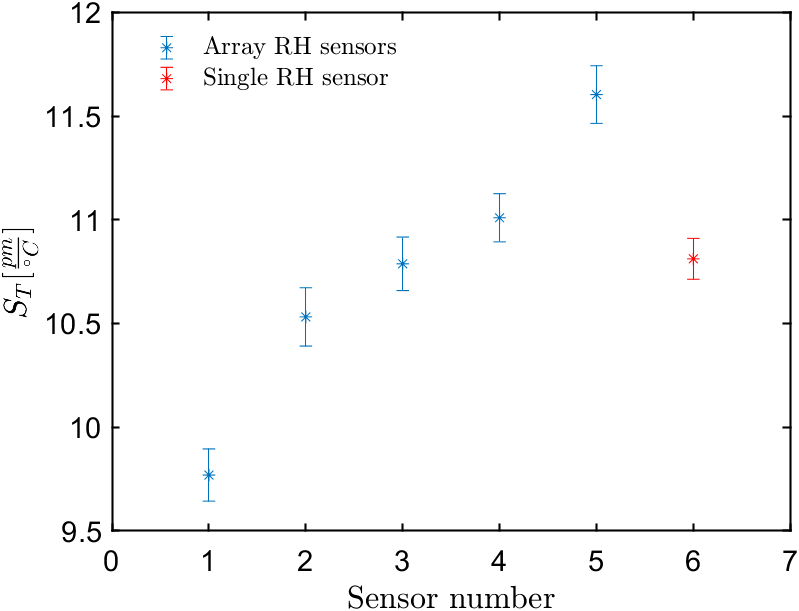
\includegraphics[width=0.6\columnwidth]{Chapter5/images/comp.png}
\caption{Hysteresis}
\label{fig_calibration}
\end{figure}


\begin{figure}[!h]
\centering
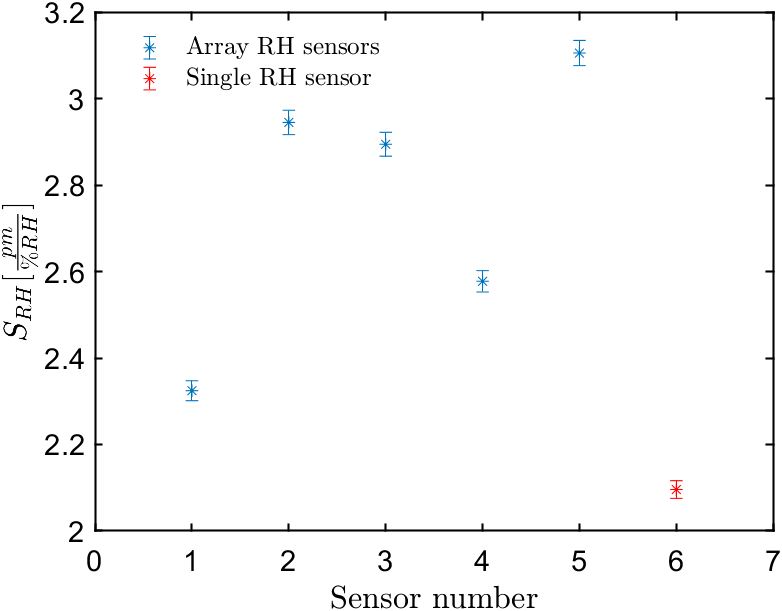
\includegraphics[width=0.6\columnwidth]{Chapter5/images/comp1.png}
\caption{Hysteresis}
\label{fig_calibration1}
\end{figure}





\subsection{Time response}

\begin{figure}[!h]
\centering
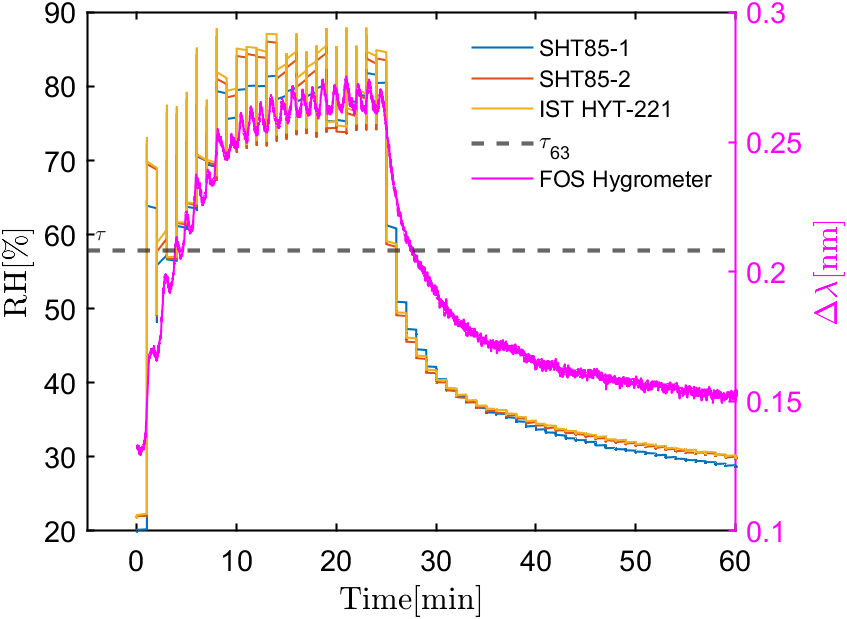
\includegraphics[width=0.6\columnwidth]{Chapter5/images/20responseRH.png}
\caption{Time response of sensors}
\label{fig_time_response}
\end{figure}

\begin{figure}[!h]
\centering
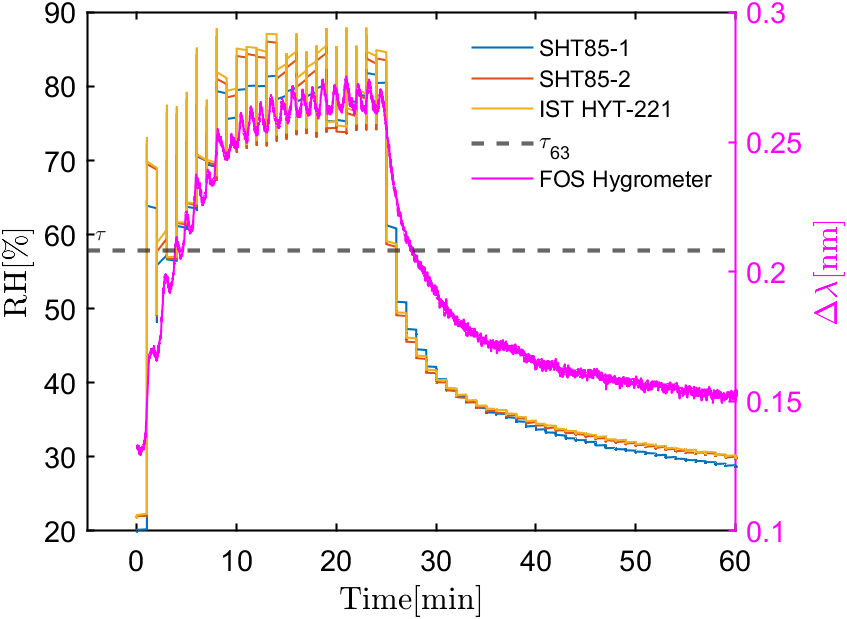
\includegraphics[width=0.6\columnwidth]{Chapter5/images/20responseRH.png}
\caption{Time response of sensors}
\label{fig_time_response2}
\end{figure}


\subsection{Hysteresis}

\begin{figure}[!h]
\centering
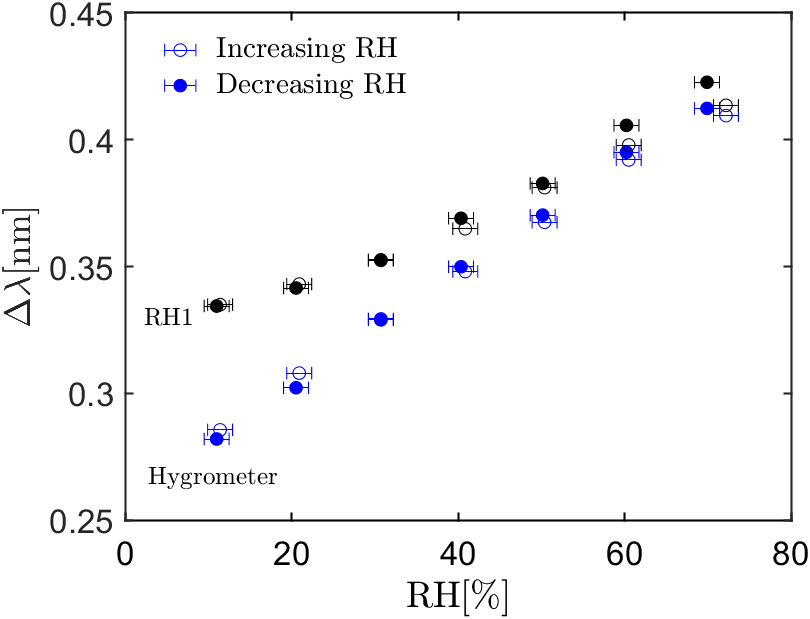
\includegraphics[width=0.6\columnwidth]{Chapter5/images/25_RHS.png}
\caption{Hysteresis}
\label{fig_hysteresis}
\end{figure}

\begin{figure}[!h]
\centering
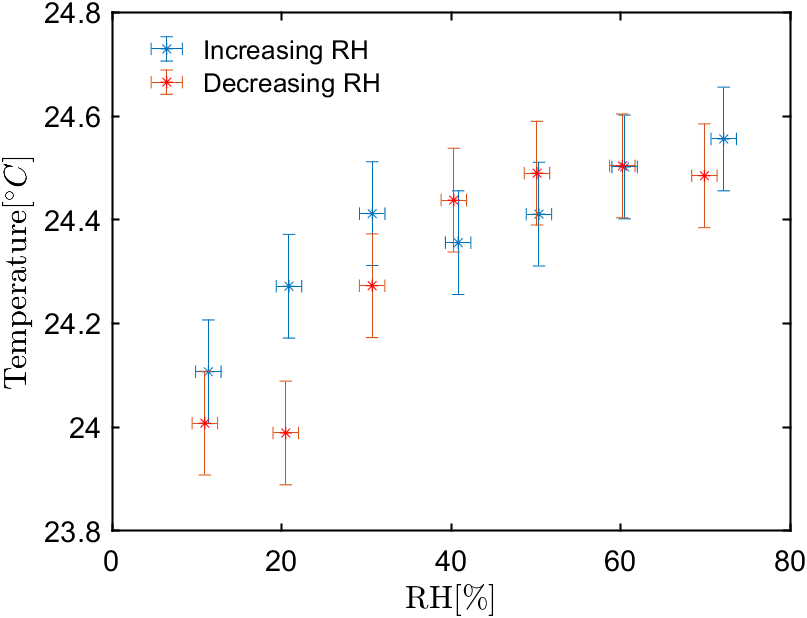
\includegraphics[width=0.6\columnwidth]{Chapter5/images/25_RHST.png}
\caption{Hysteresis}
\label{fig_hysteresis2}
\end{figure}



\subsection{Repeatability}


\begin{figure}[!h]
\centering
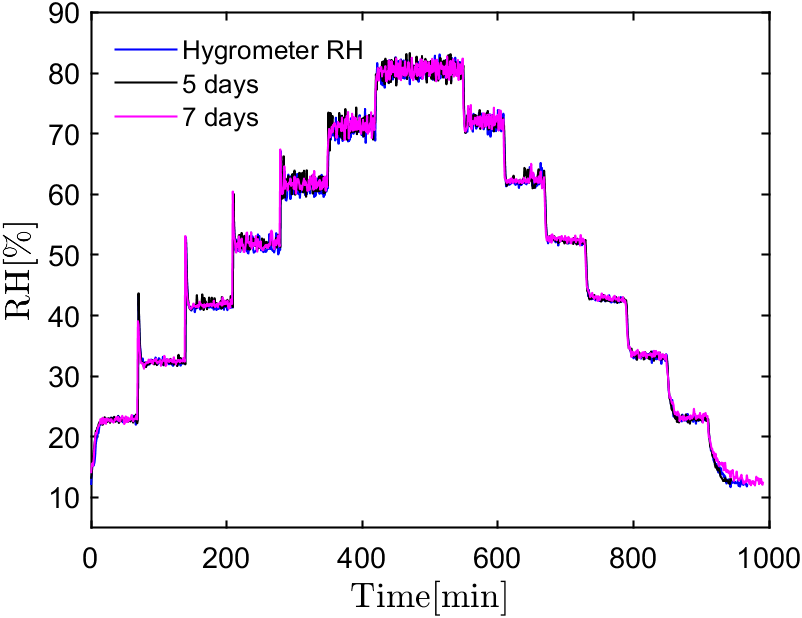
\includegraphics[width=0.6\columnwidth]{Chapter5/images/repeat.png}
\caption{Repeatability}
\label{fig_repeatability}
\end{figure}



\subsection{Conclusions}


\begin{figure}[!h]
\centering
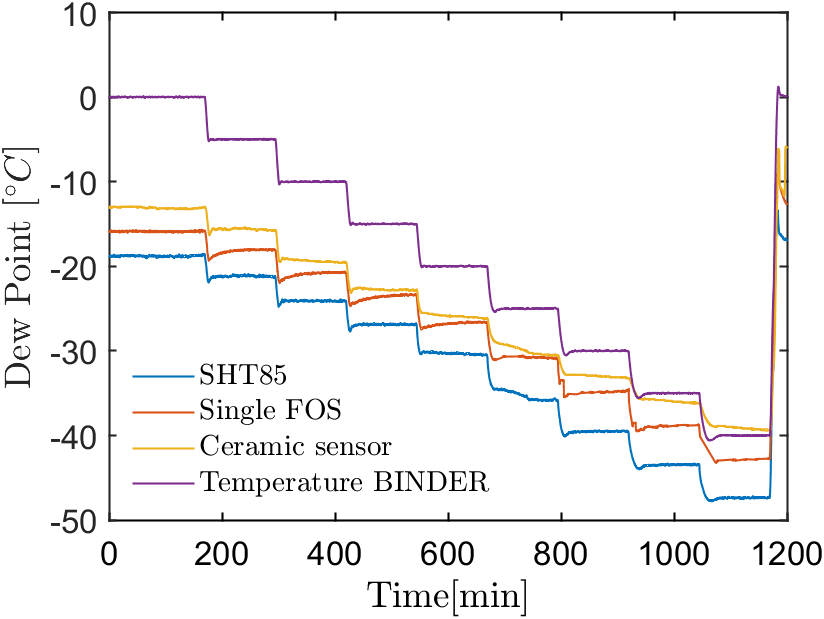
\includegraphics[width=0.6\columnwidth]{Chapter5/images/DPCPercent.png}
\caption{Comparison}
\label{fig_comparison}
\end{figure}

\begin{figure}[!h]
\centering
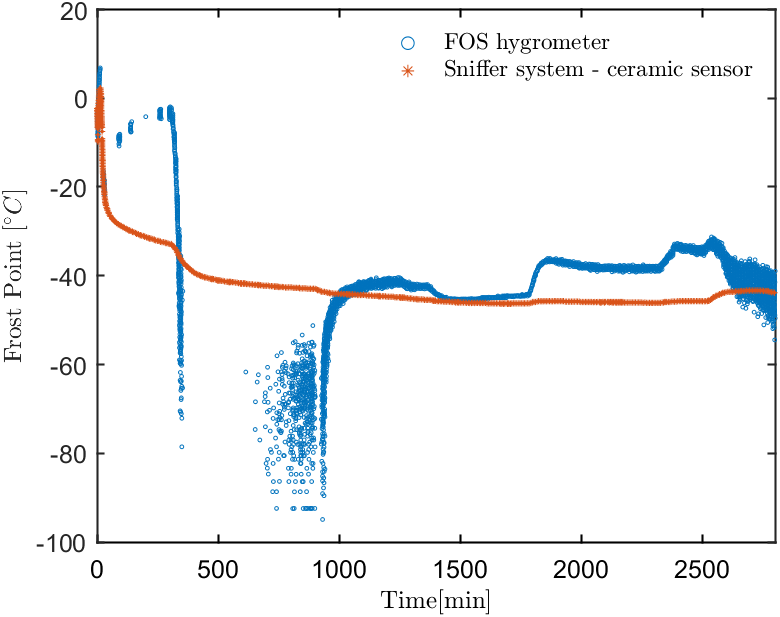
\includegraphics[width=0.6\columnwidth]{Chapter5/images/FOS_performance.png}
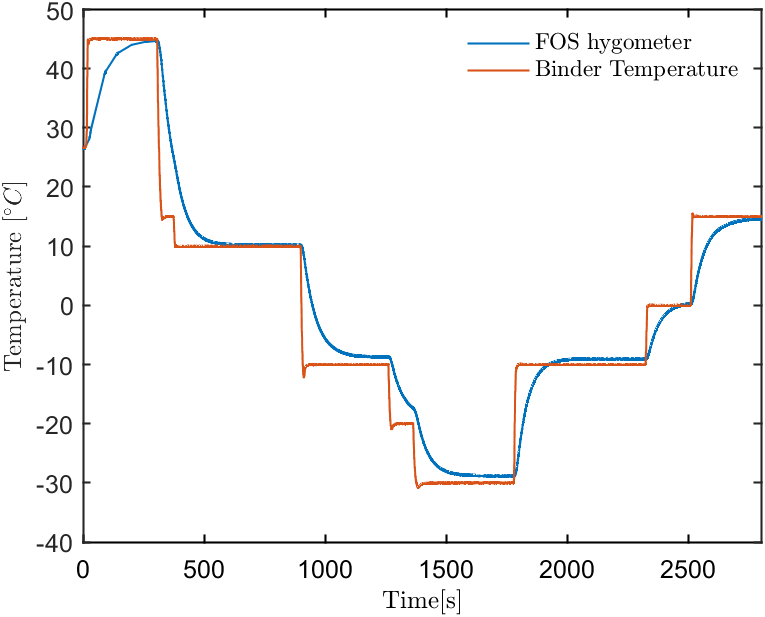
\includegraphics[width=0.6\columnwidth]{Chapter5/images/FOS_performance_T.png}
\caption{Comparison}
\label{fig_comparison1}
\end{figure}